\chapter{Software Implementierung}

\section{PX4} \label{px4:subsection}
PX 4 ist eine Open-Source-Software, welche zur Steuerung verschiedener Arten von Fahrzeugen genutzt werden kann, hierzu zählen beispielsweise verschiedene Drohnenarten, sowie auch Fahrzeuge auf dem Boden und Unterwasserfahrzeuge.\\ Es kann zum einen für bereits flugfähigen Drohen eingesetzt werden. Aber es besteht auch die Möglichkeit eine neue Drohne in Verbindung mit PX4 zu bauen.\\
Für die Verwendung der PX4 Software kann QGroundControl (siehe Kapitel \ref{qGroundControl:subsection}) verwendet werden. \cite[vgl.][]{px4} \\
Der PX4-Flugstack wurde ursprünglich nur dür die Pixhawk-Hardware entwickelt, allerdings ist es heutzutage auch möglich diesen auf Linux-Computern und anderen Hardware einzusetzen. Wie es auch bei der Coex Clover Drohne mit dem Coex Pix umgesetzt wird. \\
Die Software setzt Sensoren, ein um den Zustand der Drohne zu bestimmen. Hierfür werden einige Sensoren vorausgesetzt, zu diesen zählen ein Gyroskop, ein Beschleunigungssensor, ein Magnetometer sowie ein Barometer. Zudem ist GPS empfohlen um weitere Modi nutzen zu können. \cite[vgl.][]{px4}

\subsection{Flugmodi}
PX4 bietet verschiedene Flugmodi an, welche das Verhalten der des jeweiligen Fahrzeuge beziehungsweise Drohnen steuert und auch regelt, wie jeweils auf Benutzereingaben regiert werden soll. Das Wechseln dieser Flugmodi kann zum einen über die QGroundControl Software (siehe Kapitel \ref{qGroundControl:subsection}) oder auch je nach Anpassung der Fernbedinung, beispielsweise über verschiedene Schalter, auf dieser vollzogen werden. \\
Allerdings muss auch beachtet werden, dass nicht alle Flugmodi bei allen Drohnen oder Fahrzeugen einsetzbar sind. Aussschlaggebend hierfür ist vor allem die Ausstattung des. Da jeder Flugmodi bestimmte Bedingungen hat die erfüllt sein müssen, beispielsweise Sensoren wie ein Geschwindikgeitssensor. \\
Die Flugmodi lassen sich in drei Kategorien einteilen, diese sind manuelle, ünterstütze sowie automatische Steuerung.
Da es bei diesem Projekt um den Einsatz einer Drohne handelt, werden im folgenden lediglich die für Drohnen relevanten Flugmodi erläutert.
Zu der manuellen Steuerung, bei welchem der Pilot die Drohne direkt und ohne direkte UNterstützung steuert, gehören unter anderem die Modi "manuell" beziehungsweise "stabilisiert". Diese sorgen für eine stabilisierte horizontale Ausrichtung, jedoch ermöglichen sie es dem Piloten hierbei, das Gaspedal sowie die Roll- und Neigbewegungen selbst zu bestimmen. Zu dieser Katergorie gibt es noch weitere Modi, welche allerdingsa hauptsächlich für Flugshows genutzt werden.
Bei der unterstützen Steuerung kann aus zwei verschiedenen Flugmodi gewählt werden, "ALTCTL (Altitude)" und "POSCTL (Position)". Beim ALTCTL-Modi wird besonders die Höhe der Drohne von Autopliot gesteurt, sodass diese einen möglichst konstanten Abstand zum Boden hält. Dieser Modi benötigt hierfür ein Barometer oder andere Sensoren zur Höhenmessung.
Der POSCTL dient zum Halten der Position der Drohne, das heißt neben der Höhe werden zudem die Bewegungsgeschwindkeit nach vorne, hinten und zur Seite gesteuert, um die Drohne möglichst auf einer bestimmten Position zu halten.\\
Bei der automatischen Steuerung fliegt die Drohne automatische ohne Benutzereingaben mittels eines Programms. Zu dieser Katergorie gehört der "Offboard"-Modus hierdurch ist es möglich, dass die Drohne durch einen anderen Computer gesteuert werden kann. Zudem gibt es noch einen Missions-Modus, hierbei kann beispielsweise über QGroundControl ein Pfad geplant werden, welcher dann von der Drohne mittels GPS geflogen wird. \\
Für das Projekt ist hierbei vor allem der Offboard-Modus von Bedeutung, da dieser benötigt wird, um autonome Flüge mit der Coex Clover Drohne zu machen, da diese hierbei von dem Raspberry Pi gesteuert wird. \cite[vgl.][]{flight-modes}


\subsection{QGroundControl}  \label{qGroundControl:subsection}
QGroundControl ist eine Software, welche vor allem für Drohnen mit einem PX4 aber auch anderen Flight Controller genutzt werden kann. Hierbei bietet es verschiedene Funktionen. Zum einen gehört hierzu die Konfiguration der einzelnen  Drohnen. Desweiteren ist es möglich mit der Software verschiedene Flugmodi auszuwählen, sowie diese dann auch während des Fluges zu überwachen, beispielweise durch die Anzeige der Flugposition auf einer Karte sowie auch deren Geschwindigkeit und andere Sensordaten.
Es ist auch möglich mit QGroundControl eine ganze Flugplanung zu machen, welche die Drohne daraufhin umsetzt. \cite[vgl.][]{qGroundControl}


\section{Systemarchitektur}

\section{Softwarearchitektur}
\todo{Beschreibung Mavros}

    %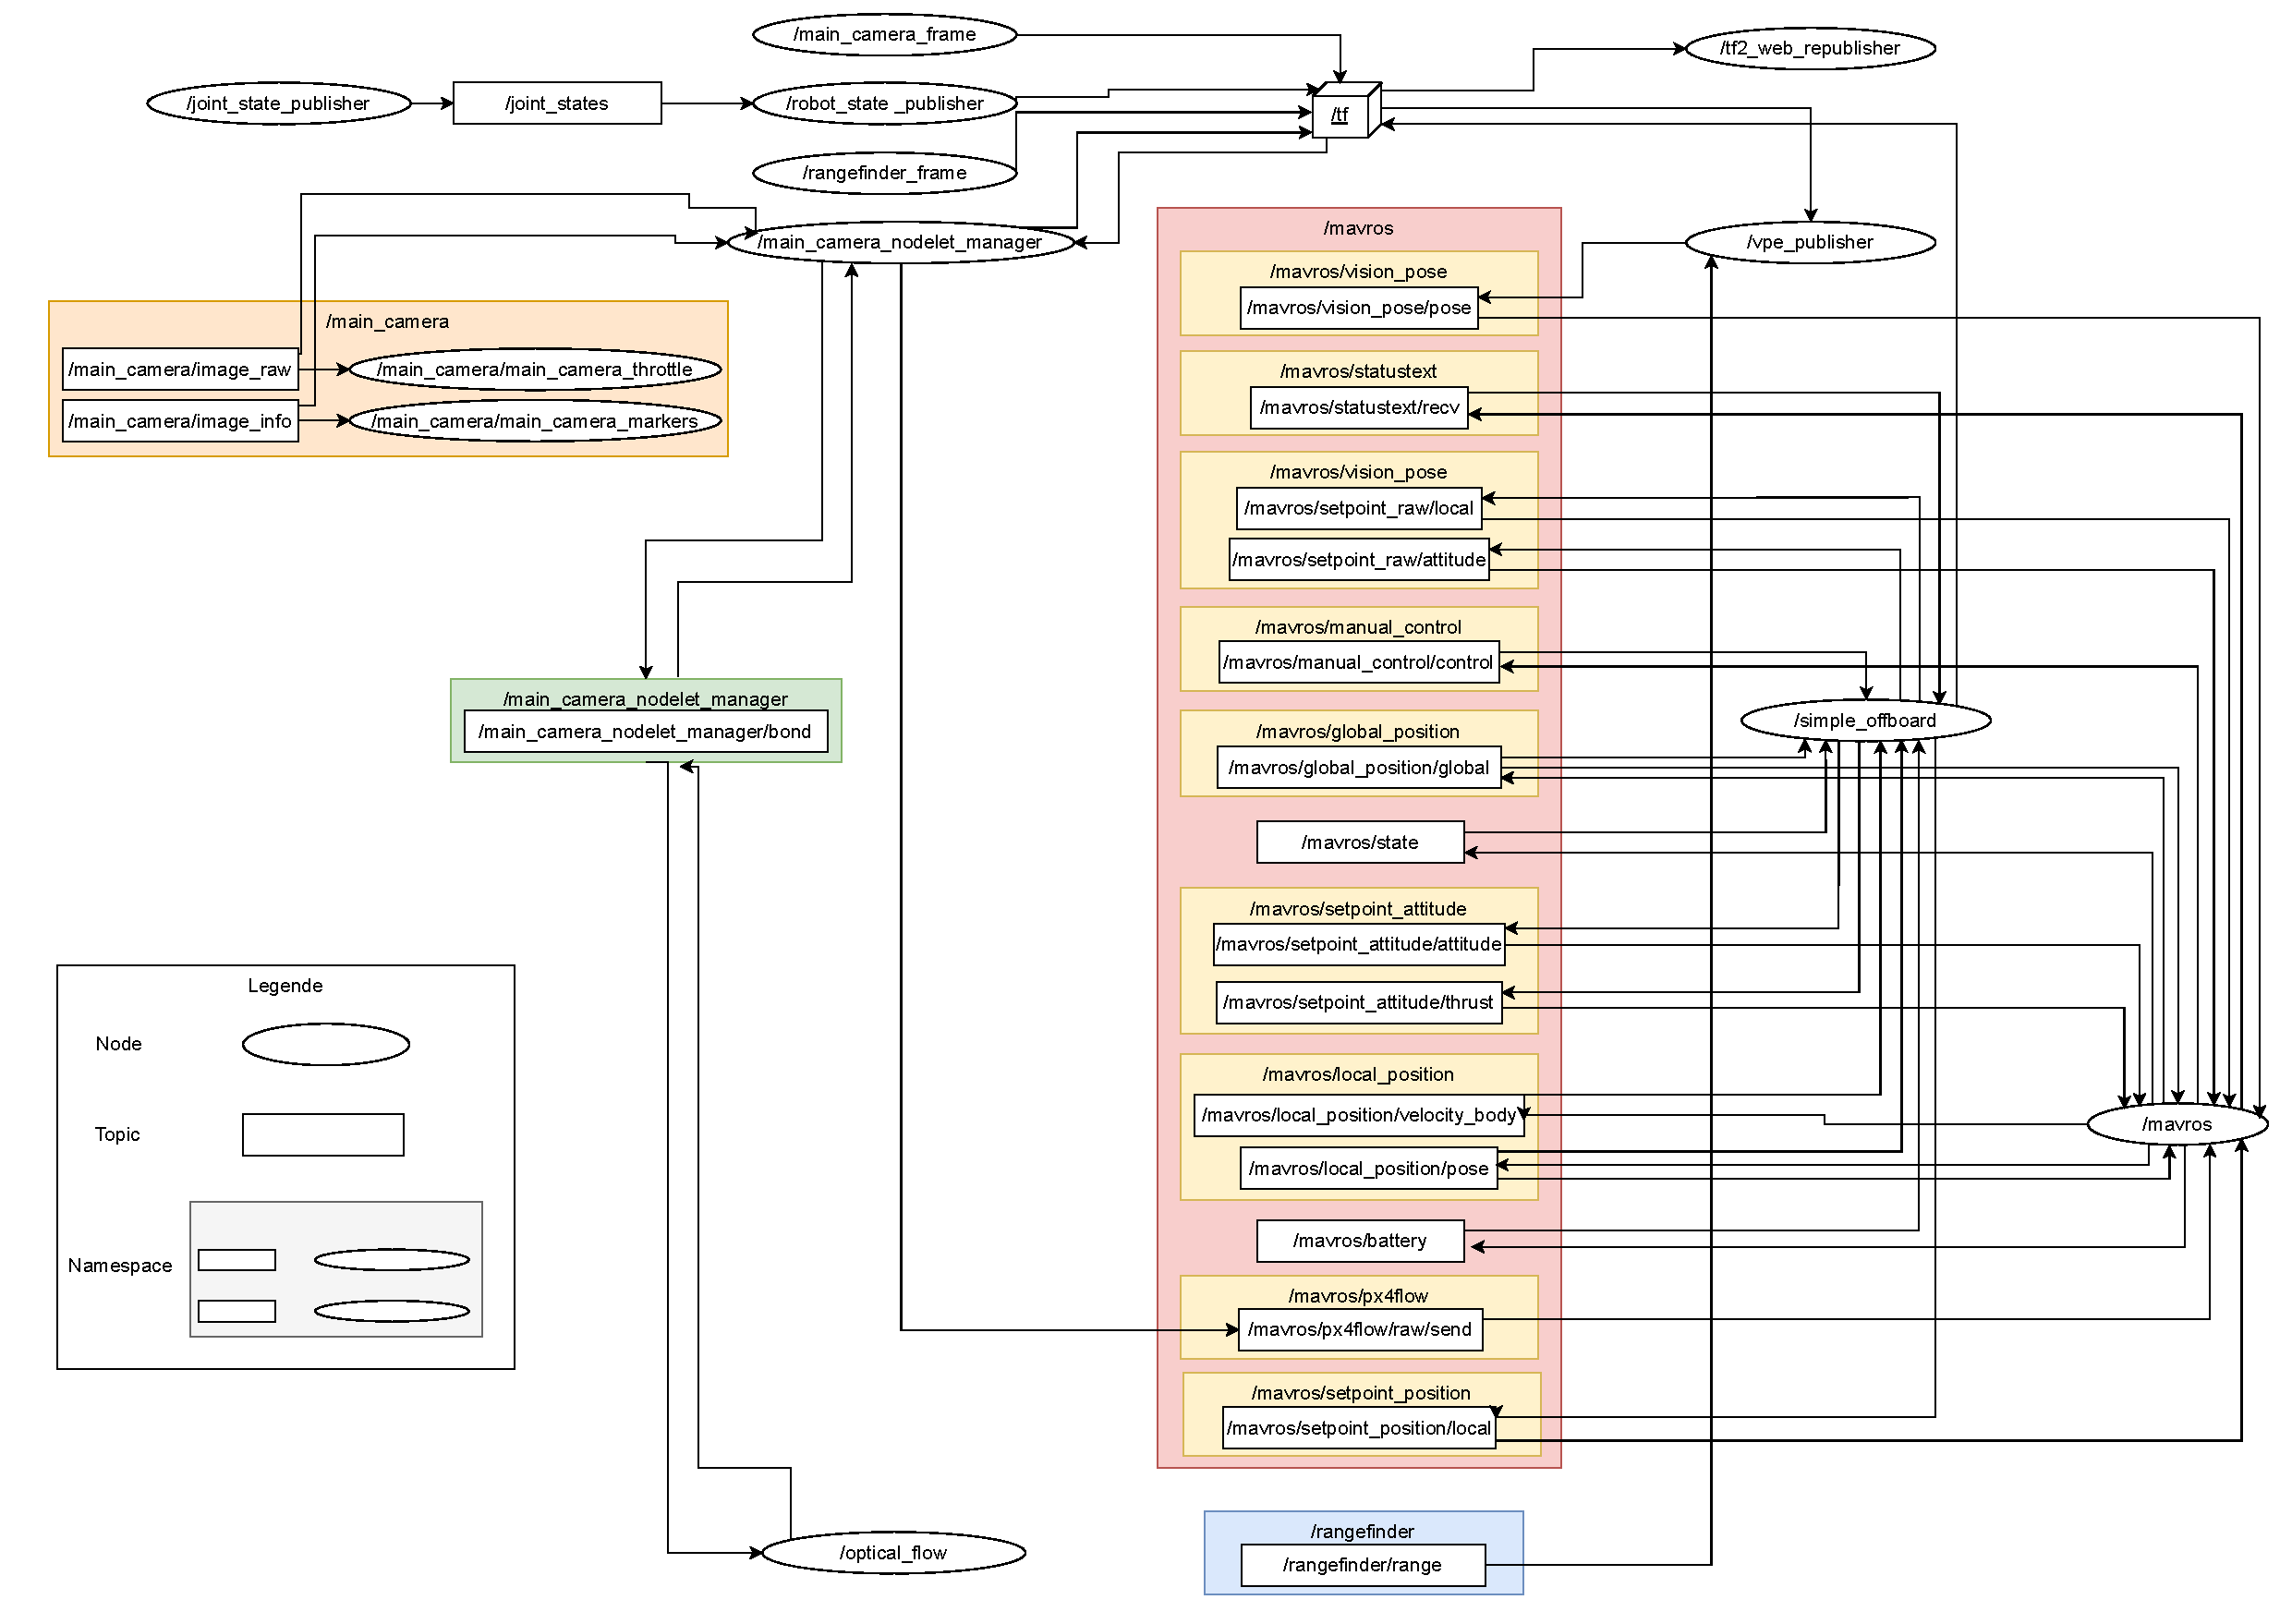
\includepdf[landscape=true]{images/graph_ros.pdf}
    %\caption[Übersicht ROS Nodes]{\label{img ros_nodes_graph} Übersicht ROS Nodes [eigene Darstellung]}
    \begin{landscape}
        \begin{figure}
            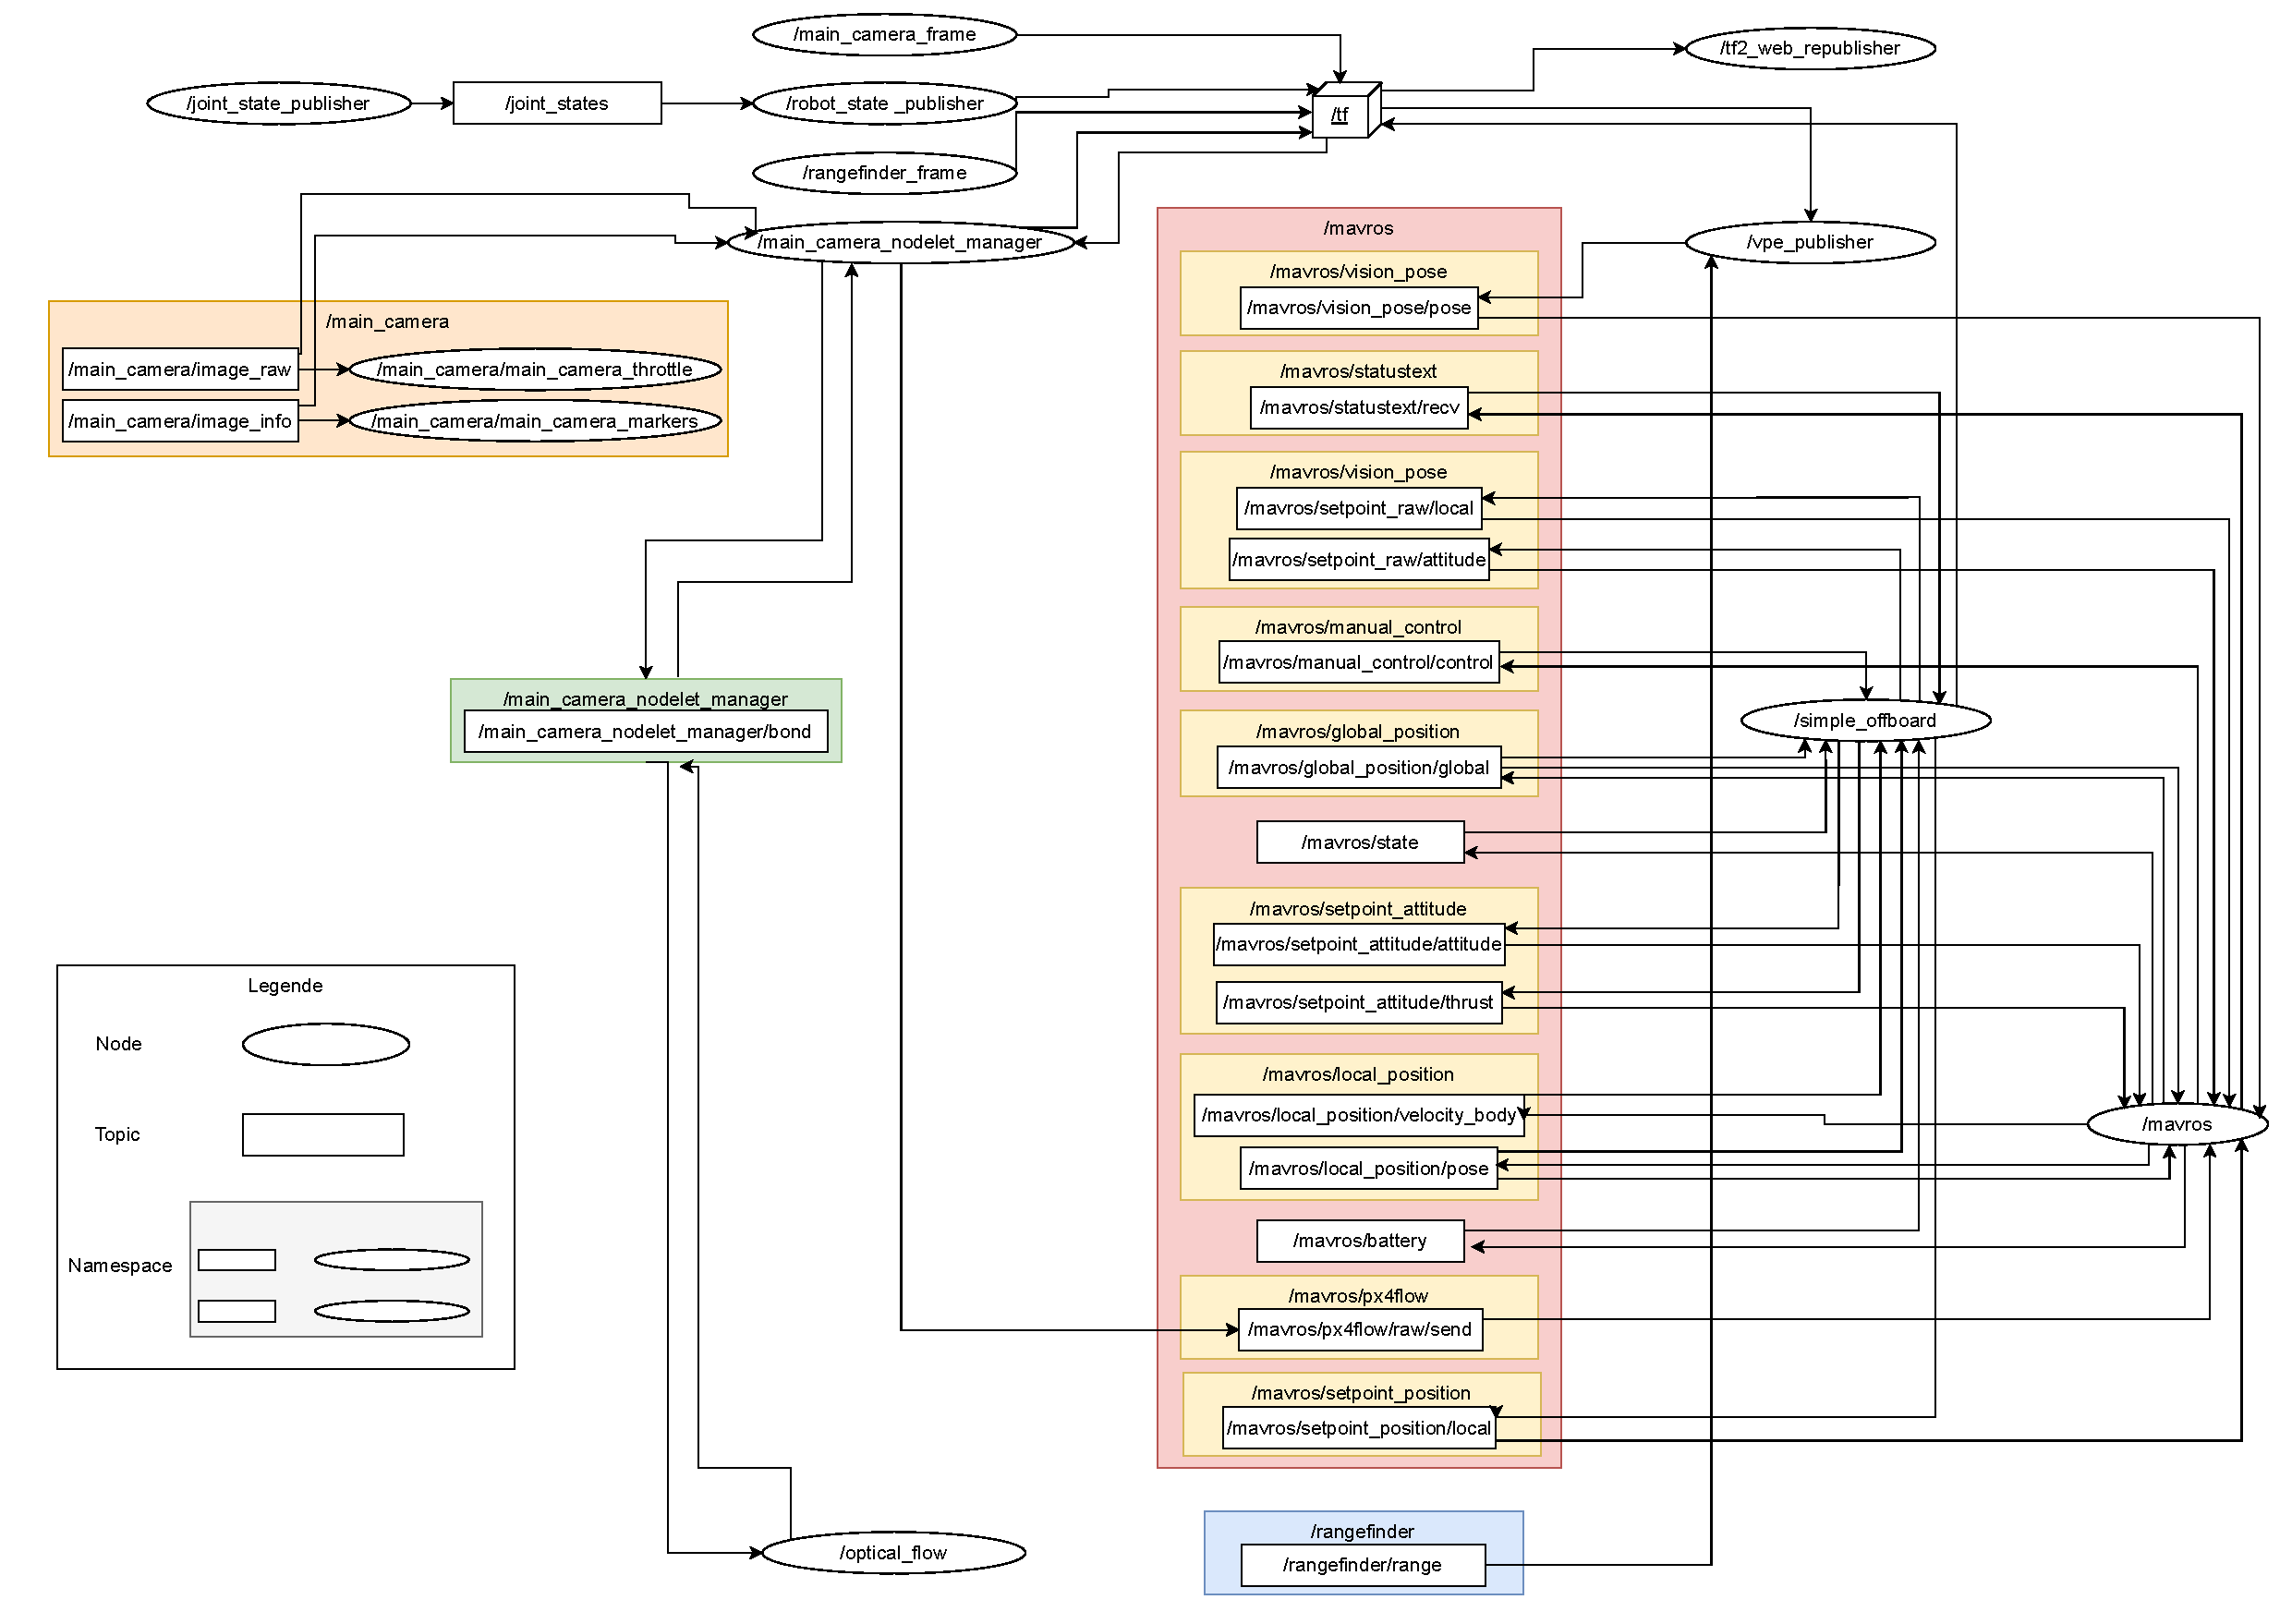
\includegraphics[width=\paperwidth,keepaspectratio]{images/graph_ros.pdf}
            \caption[Übersicht ROS Kommunikation]{\label{img ros_communication} Übersicht ROS Kommunikation [eigene Darstellung]}
        \end{figure}
    \end{landscape}

In der Abbildung \ref{img ros_communication} ist eine Übersicht der Kommunikation zwischen den verschiedenen Komponenten in \ac{ROS} zu sehen. \\
Hauptbestandteil sind hierbei vor allem die Nodes der Hauptkamera beziehungsweise der Azure Kinect sowie auch Mavros. \\
Mavros ist hierbei ein ROS-Paket, welches die Kommunikation zwischen dem Raspberry Pi und der Drohne mit Hilfe des MAVLink-Protokolls (siehe Kapitel \ref{mavlink}) ermöglicht. Es unterstützt dabei unter anderem den PX4 Flightstack, welcher in der Coex Clover Drohne vorhanden ist. Die Kommunikation kann hierbei wie bei MAVLink auch über \ac{USB} oder auch über Wifi stattfinden. \\
Im nachfolgenden wird nun genauere auf einzelne Komponenten der ROS Kommunikation (siehe \ref{img ros_communication}) eingegangen. \\

%https://clover.coex.tech/en/mavros.html


\section{Kalibrierung der COEX Drohne}

\section{Drohnen Autopilot}


\section{3D Modell}
Um die Drohne auch in der Simulation unter echten Bedingungen fliegen zu lassen, müssen die realen Gegebenheiten in die Simulation übertragen werden. Um dies zu bewerkstelligen, muss ein 3D-Modell der Räume erstellt werden, in welchen sich die Drohne bewegen soll.
    \subsection{3D Scan}

        \subsubsection{Microsoft HoloLens 2}
        Um ein 3D-Modell des Raumes mit der Microsoft HoloLens 2 zu erstellen, muss man die integrierte Mixed-Reality-Capture-Funktion der HoloLens 2 verwenden.
        
        Die Mixed-Reality-Capture-Funktion der HoloLens 2 ist eine integrierte Funktion, mit der Benutzer die Möglichkeit haben, die Hologramme, die von der HoloLens 2 dargestellt werden, in Echtzeit aufzuzeichnen und zu teilen. Diese Funktion ermöglicht es Benutzern, ihre Augenbewegungen und Handlungen in einer virtuellen Umgebung aufzuzeichnen, um sie mit anderen zu teilen oder für zukünftige Referenz oder Analyse zu speichern. Die Mixed-Reality-Capture-Funktion der HoloLens 2 kann auch für die Erstellung von Immersive-Mixed-Reality-Videoinhalten verwendet werden, indem sie es ermöglicht, virtuelle Hologramme in eine reale Umgebung zu integrieren. Dies kann für verschiedene Anwendungen wie zum Beispiel für die Erstellung von virtuellen Touren, für die Präsentation von Produkten oder für die Unterhaltungsindustrie eingesetzt werden.
        
        \todo{Erstellen des Modells beschreiben}

        Es ist wichtig zu beachten, dass die Qualität des erstellten 3D-Modells von verschiedenen Faktoren abhängt, wie z.B. der Beleuchtung im Raum und der Genauigkeit des Scans. Eine sorgfältige Vorbereitung des Raums und eine langsame, gründliche Durchführung des Scans können dazu beitragen, ein genaueres und detaillierteres 3D-Modell zu erstellen.
        \subsubsection{Azure Kinect \ac{DK}}

    \subsection{3D Modell Vorbereitung}

\section{Navigation}

\section{Simulation}



